% !TEX TS-program = pdflatex
\documentclass[11pt]{article}
\usepackage[margin=1in]{geometry}
\usepackage{amsmath,amsfonts}
\usepackage{hyperref}
\usepackage{graphicx}
\usepackage{authblk}
\usepackage{booktabs}
\usepackage{enumitem}
\usepackage{xcolor}

\title{\bf Semantic Tensor Memory: A Structured Memory System for Tracking Meaning Across Time, Tokens, and Context}

\author[1]{Joshua Farrow\thanks{Correspondence: joshuajamesfarrow@gmail.com}}
\affil[1]{Independent Researcher, Richmond, VA, USA}

\date{Draft -- June 2025}

\begin{document}
\maketitle

\begin{abstract}
We introduce \emph{Semantic Tensor Memory} (STM), a structured, interpretable memory system for tracking evolving meaning across time, tokens, and context. Unlike traditional flat vector stores, STM preserves a three-dimensional tensor of token-level embeddings over sequential conversation steps or document windows---enabling granular analysis of semantic drift, relational clustering, and transparent, modular storage. We formalize the STM architecture, present robust visualization and drift quantification techniques, and demonstrate applications in both clinical analytics and financial market intelligence. STM establishes a foundation for next-generation memory models in AI, offering interpretable, longitudinal insight for research, autonomous agents, and real-world decision support.
\end{abstract}
    

\section{Introduction}
Modern AI systems---from large language model (LLM) chatbots to clinical assistants and financial analytics engines---increasingly depend on external memory systems to maintain context, enable retrieval-augmented generation (RAG), and track evolving user or market intent. However, most contemporary architectures rely on either a limited context window or flat vector stores, both of which summarize text at the sentence or chunk level. This approach misses the fine-grained, temporal evolution of meaning that is often critical not only in healthtech and coaching, but also in high-stakes domains such as financial market intelligence, regulatory monitoring, and narrative-driven investing.

We propose \textbf{Semantic Tensor Memory (STM)}: a three-dimensional tensor structure that stores the sequence of token embeddings per conversation turn or document window, providing a granular and interpretable representation of semantic change over time. STM empowers downstream agents---including LLMs and market analytics pipelines---to reason over not just ``what'' was said, but ``how'' meaning and context have shifted across time, transactions, or narratives.

By moving beyond static recall toward a dynamic, drift-aware memory, STM opens new possibilities for longitudinal analysis in healthtech, interpretable LLM agents, and real-time narrative monitoring in finance and other high-impact verticals.

\section{Related Work}
\begin{itemize}[leftmargin=2em]
    \item \textbf{Vector databases and RAG:} Tools like Pinecone, Chroma, and LangChain enable retrieval-augmented LLMs, but focus on document or chunk-level retrieval.
    \item \textbf{Memory-augmented neural networks:} Prior work (e.g., Differentiable Neural Computers, Transformer-XL) explores learnable tensor memories, but lacks user-facing interpretability.
    \item \textbf{Semantic drift and behavioral analytics:} Behavioral science has long sought tools to monitor change in client language or intent, but current NLP applications rarely reach token-level granularity.
\end{itemize}

\section{STM Architecture}
Let $T$ denote the number of conversation steps, $N_t$ the number of tokens in step $t$, and $D$ the embedding dimension. STM stores each session as a list of tensors $\{M_t\}_{t=1}^T$ where $M_t \in \mathbb{R}^{N_t \times D}$ is the embedding of tokens in step $t$.

\vspace{0.5em}
\textbf{Construction:}
\begin{enumerate}[leftmargin=2em]
    \item Tokenize each input with a transformer model (e.g., BERT).
    \item For each step $t$, extract the last hidden state, yielding $N_t \times D$ token embeddings.
    \item Store each step's embeddings as a separate tensor in the session list.
    \item Attach metadata: timestamps, user IDs, context tags, and any additional columns from imported data.
\end{enumerate}

\vspace{0.5em}
\textbf{Implementation (PyTorch):}
\begin{verbatim}
# For each step:
inputs = tokenizer(sentence, return_tensors="pt")
with torch.no_grad():
    outputs = model(**inputs)
memory_list.append(outputs.last_hidden_state)  # Store as-is

# For analysis (batch-on-demand):
batch = pad_and_stack(memory_list)  # Pad only when needed
valid_mask = (batch != 0).all(dim=-1)  # Mask padded rows
\end{verbatim}

\vspace{0.5em}
\textbf{Data Import:}
STM supports both interactive session input and CSV import. For CSV files, a GUI file picker enables selection, and all columns are preserved as metadata alongside the embedded text column. This ensures reproducibility and maintains the full context of each session.

\section{Visualization and Drift Metrics}
STM enables rich semantic analytics with robust preprocessing and interpretable outputs:

\begin{itemize}[leftmargin=2em]
    \item \textbf{Robust PCA/UMAP projections:} Before dimensionality reduction, padded rows and numerical instabilities (NaN, Inf) are masked out. Data is normalized, and diagnostics report the proportion of valid vs. masked rows. This ensures stable, interpretable projections of token-level clusters and their temporal drift.
    
    \item \textbf{Session mean trajectories:} Compute mean embedding per step (excluding masked rows) to trace a user's semantic trajectory through latent space.
    
    \item \textbf{Cosine drift heatmaps:} Quantify semantic change between steps using pairwise cosine distances, with optional masking of invalid comparisons.
    
    \item \textbf{LLM-powered interpretation:} Local language models (e.g., via Ollama) generate clinical summaries and interpret principal axes by analyzing outlier tokens and associated keywords. This bridges quantitative drift metrics with narrative understanding.
\end{itemize}

\begin{figure}[h]
    \centering
    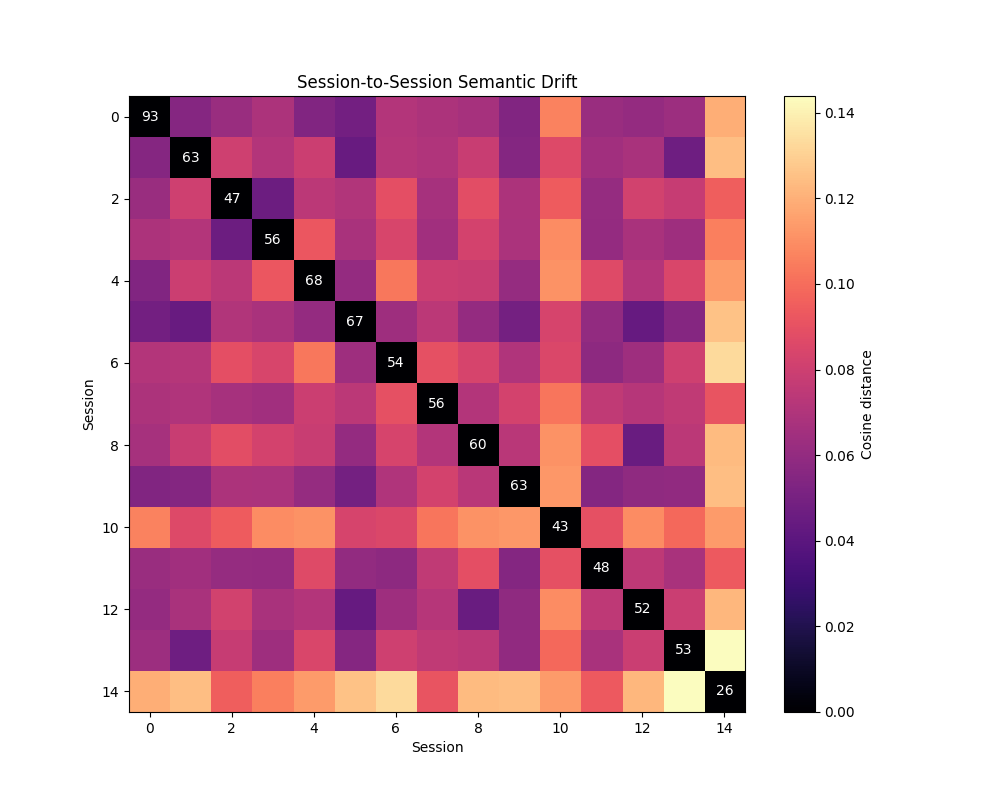
\includegraphics[width=0.7\textwidth]{demo_session-to-session_semantic_drift.png}
    \caption{Session-to-session semantic drift visualization showing the evolution of meaning across multiple conversation turns. The heatmap reveals patterns of semantic stability and change over time.}
    \label{fig:drift}
\end{figure}

\begin{figure}[h]
    \centering
    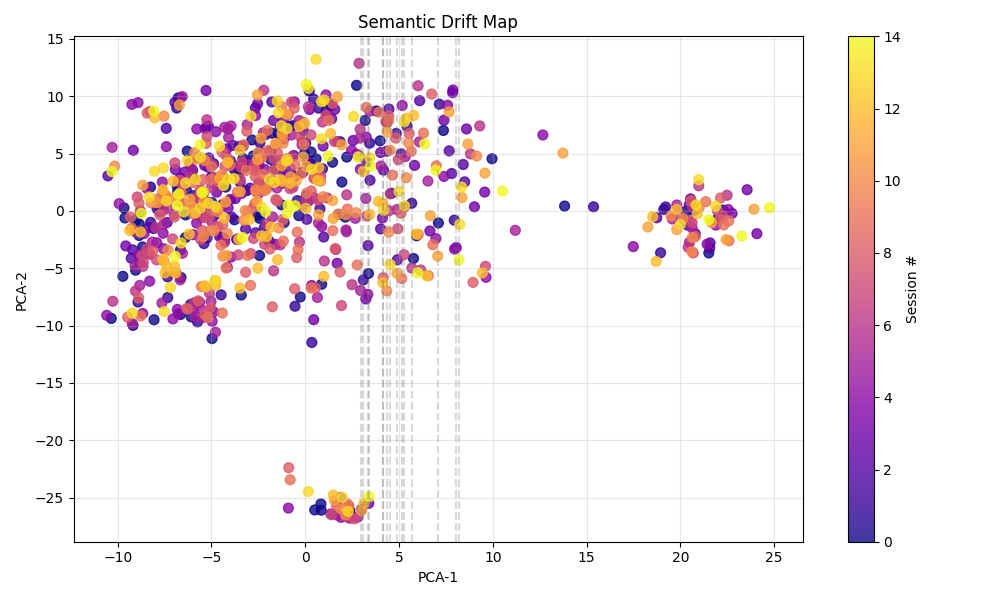
\includegraphics[width=0.7\textwidth]{demo_drift_map.png}
    \caption{Detailed drift map illustrating token-level semantic changes. The visualization highlights how individual tokens shift in meaning across the conversation timeline.}
    \label{fig:drift_map}
\end{figure}

\section{Applications}

\subsection{Financial Market Intelligence and Narrative Drift}
STM empowers real-time tracking of evolving narratives in financial news, social media, and regulatory commentary. By embedding headlines and reports into a temporal semantic tensor, STM quantifies shifts in sentiment, risk perception, and theme rotation—surfacing regime changes and actionable signals ahead of price movements. Portfolio managers and quant funds can leverage STM outputs for event detection, risk mitigation, and narrative-based alpha generation.

\subsection{Brand Monitoring and Social Listening}
STM detects semantic drift in consumer conversations, product reviews, and media coverage—enabling brands to monitor shifts in perception, emerging trends, or potential crises. Marketers and PR teams can use STM analytics to adjust messaging, benchmark competitors, and intervene before negative narratives gain traction.

\subsection{Healthtech, ABA, and Clinical QA}
STM provides early warning of documentation drift in clinical notes or behavioral session logs, supporting proactive interventions in autism, ADHD, mental health, and quality assurance. Token-level tracking reveals subtle changes in patient status, adherence to protocols, or compliance risks, supplementing traditional audit tools with interpretable visualizations and alerts.

\subsection{Reflective LLM Agents and Autonomous Systems}
STM serves as an external memory for LLM-based agents, capturing not just what was said, but how meaning and intent have changed over time. This enables narrative coherence, meta-cognitive reasoning, and reflective feedback loops in conversational AI, customer support bots, or legal research assistants.

\subsection{Education, Coaching, and Human Development}
Longitudinal STM maps learning trajectories for students or clients, enabling adaptive instruction, personalized feedback, and the early detection of conceptual or motivational drift. Educators and coaches can visualize progress and tailor interventions for maximum growth.

\section{Example Analysis: ABA Session Notes}

To illustrate STM's interpretability, we present an analysis of ABA session notes from a 3-year-old with emerging speech, aggressive behavior, and elopement concerns. The STM pipeline yields principal component axes (PCA-1, PCA-2) and automated clinical summaries.

\subsection{PCA Output and Interpretation}

\textbf{Explained Variance:} PCA-1: 7.7\%, PCA-2: 6.6\%

\textbf{Axis Analysis:}
\begin{itemize}[leftmargin=2em]
    \item \textbf{PCA-1 (Engagement \& Communication):} 
    \begin{itemize}
        \item \textbf{Positive:} Calm participation, no aggression/elopement, spontaneous requests, independent imitation.
        \item \textbf{Negative:} Increased engagement with picture cards, single-word requests, aggression during cleanup, elopement attempt, hand-over-hand imitation.
    \end{itemize}
    \item \textbf{PCA-2 (Initiation \& Social Responsiveness):}
    \begin{itemize}
        \item \textbf{Positive:} Initiates play, two-word requests, imitation after prompts; aggression only during work demands.
        \item \textbf{Negative:} Elopement on doorbell, aggression during cleanup, spontaneous requests, imitation only with full prompt.
    \end{itemize}
\end{itemize}

\subsection{Clinical Analysis Summary}
\begin{itemize}[leftmargin=2em]
    \item \textbf{Axis 1:} Reflects engagement, spontaneous communication, and imitation; negatives mark frustration, sensory overload, or difficulty with transitions.
    \item \textbf{Axis 2:} Captures initiation and social responsiveness; positives show reciprocity, negatives highlight regulation or environmental triggers.
    \item \textbf{Key Patterns:} Spontaneous requests (``cookie,'' ``car''), imitation, aggression during demands, elopement on transitions, initiating play.
    \item \textbf{Transitions:} Decreased aggression during cleanup, shift from hand-over-hand to independent imitation, improved elopement management.
    \item \textbf{Significance:} Indicates progress in self-regulation, communication, and social learning, with ongoing need for targeted intervention.
\end{itemize}

\begin{figure}[h]
    \centering
    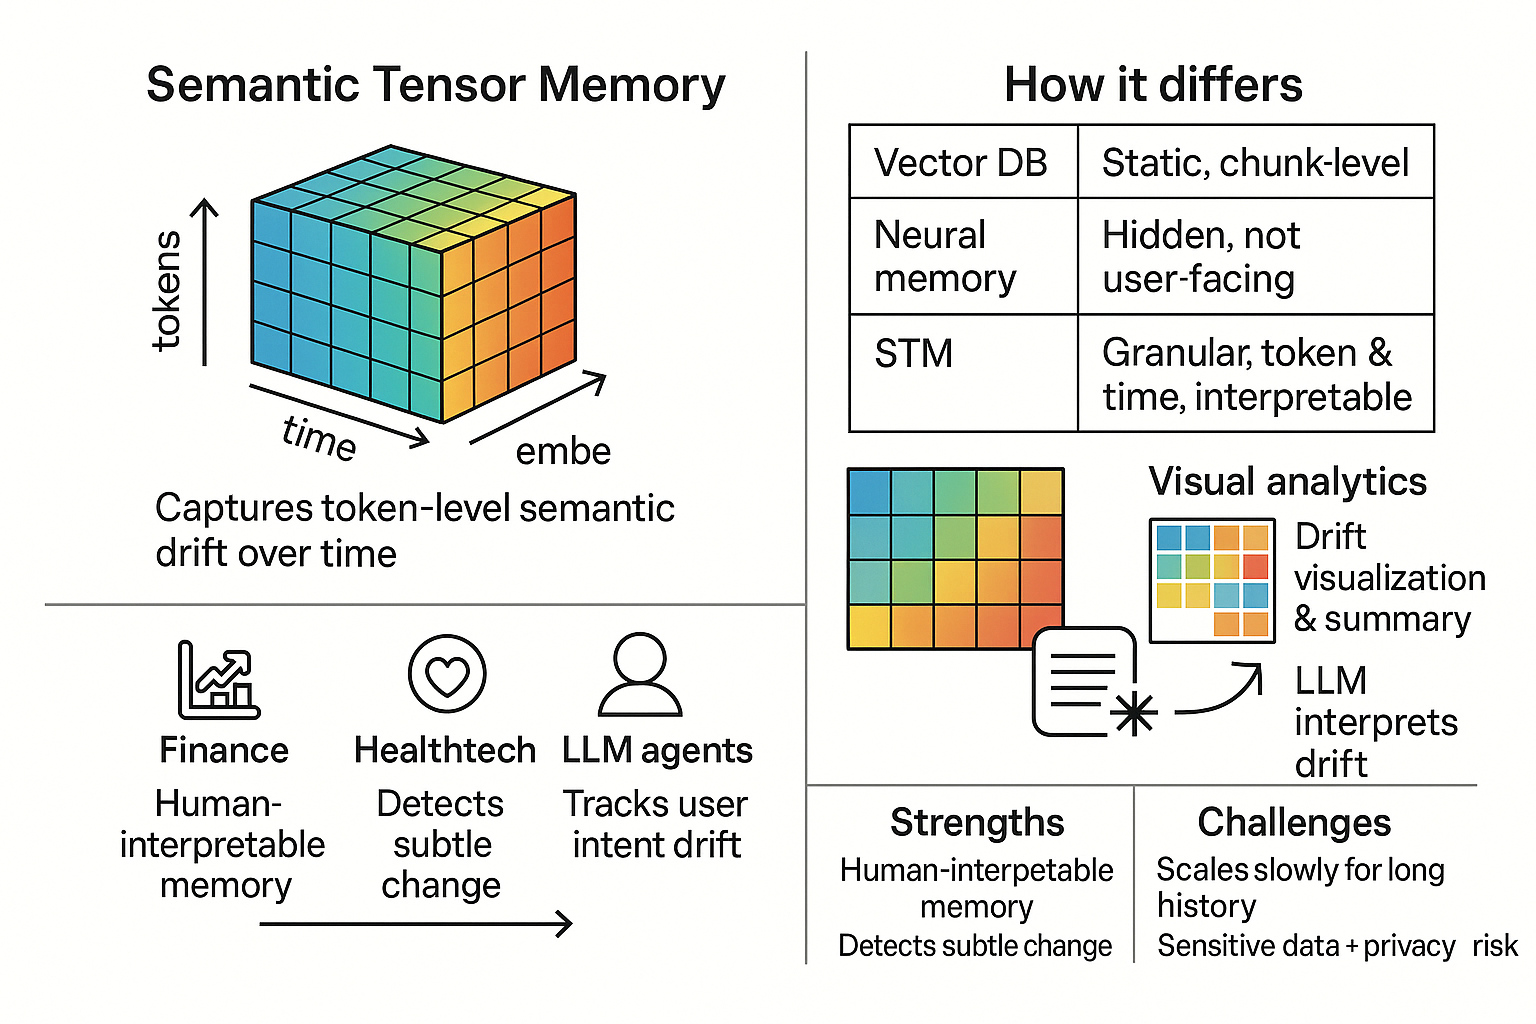
\includegraphics[width=0.7\textwidth]{summary_image.png}
    \caption{Summary visualization of ABA session analysis. This figure provides an overview of key patterns and transitions identified in the session data.}
    \label{fig:summary}
\end{figure}

\section{Limitations and Future Work}
\begin{itemize}[leftmargin=2em]
    \item \textbf{Embedding model dependence:} STM quality depends on the expressivity of underlying transformer embeddings. Current implementation uses BERT, but could be extended to other models.
    
    \item \textbf{Memory efficiency:} While ragged storage is more efficient than fixed-size tensors for variable-length sessions, long-term storage of many sessions may require compression or summarization techniques.
    
    \item \textbf{LLM integration:} Current implementation uses local LLMs (via Ollama) for interpretation and summaries. Future work could explore direct tensor-to-LLM interfaces for more sophisticated reasoning over semantic drift.
    
    \item \textbf{Privacy and governance:} Token-level memory may expose sensitive semantic drift. Future work should explore privacy-preserving techniques and governance frameworks for clinical applications.
    
    \item \textbf{Edge cases:} While the system handles common edge cases (variable length, missing data, numerical instability), more sophisticated error recovery and validation could improve robustness.
    
    \item \textbf{Reproducibility:} Current implementation ensures reproducibility through modular design and clear CLI interfaces, but could benefit from containerization and automated testing.
\end{itemize}

\section{Conclusion}
Semantic Tensor Memory reframes AI memory from static recall to the continuous evolution of meaning---enabling interpretable, clinically relevant, and narratively coherent memory architectures. STM stands to advance AI safety, clinical transparency, and self-reflective agent design.

\section*{Acknowledgments}
Thanks to my wife, family, and friends for their support and encouragement.

\bibliographystyle{plain}
\bibliography{stm_refs}

\end{document}
